\documentclass[conference]{IEEEtran}
%\documentclass[12pt]{article}
\usepackage{graphicx,cite,bm,psfrag,amsmath}
\def\mmax{\mathop{\mbox{\scriptsize max}}}
\def\argmin{\mathop{\mbox{arg\,min}}}
\def\argmax{\mathop{\mbox{arg\,max}}}
\newcommand{\defequal}{\stackrel{\mathrm{def}}{=}}
\renewcommand{\vec}[1]{{\ensuremath{\boldsymbol{#1}}}}
\newcommand{\popt}{\ensuremath{P^{(K)}_{opt}}}

\pagestyle{plain}
\usepackage{amsfonts}
\usepackage{algorithm, algorithmic}
\renewcommand{\algorithmicrequire}{ \textbf{Input:}} %Use Input in the format of Algorithm
\renewcommand{\algorithmicensure}{ \textbf{Procedures:}} %UseOutput in the format of Algorithm
% correct bad hyphenation here
%\hyphenation{op-tical net-works semi-conduc-tor}
\usepackage{CJK}
\usepackage{color}
\usepackage{url}
\usepackage{geometry}
\geometry{left=0.55in, right=0.7in, top=0.75in, bottom=0.75in}

\begin{document}
\title{SIR-Based Power Control Used in CDMA Systems}
\author{\IEEEauthorblockN{Wentao Liu, Guanchong Niu and Man-On Pun\IEEEauthorrefmark{3}
%\IEEEauthorrefmark{3},
\IEEEauthorblockA{
School of Science and Engineering\\
The Chinese University of Hong Kong, Shenzhen\\
Shenzhen, Guangdong, China, 518172}}}


\maketitle \thispagestyle{plain}
\pagenumbering{gobble}


% make the title area
\maketitle

% As a general rule, do not put math, special symbols or citations
% in the abstract
\begin{abstract}
	This passage summarizes some results on signal to interference (SIR) based power control algorithms The classic works of Nettleton, and Alavi attracted considerable attention in the nineties. The modern approach to the power balancing control problem in wireless networks, formulated by Zander in 1992, and made a progress in 1997. It converts the real problems into a matrix-associated questiones. 
\end{abstract}

% no keywords

\section{Introduction}
CDMA has attracted more attention to its increasing capacity. Power control is an useful way to the near-far effect in uplink and the corner effect in the downlink, so as to increase the capacity of or has an efficiency on the CDMA system.In cellular wireless communication system, an uplink specific is based on the mobile battery power.Also, downlink codes are synchronous and can be made orthogonal; but uplink codes  arrive at the base station asynchronously, resulting in cross correlation, and causing high in-cell interference potential unless power is controlled. For this reason we concentrate on the uplink.

Unlike the conditions in FDMA/TDMA cellular radio systems where in any cochannel set only one mobile in each cell, in CDMA cellular systems all the mobiles in each cell use the same frequency, which results in three dimensional link gain matrices. SIR balancing is not an eigenvalue problem any more unless intra-cell SIR balancing is assumed and the link gain matrices are simplified to two dimensions\cite{IEEEhowto:kopka}. An n th-power-of-distance power control law has been presented and discussed using a simple power control model. This model based on the distance from the base station has been investigated by Nettleton in [1]. He introduces the concept of SIR balancing, which yields a “fair” distribution of the interference in the sense that all users experience the same SIR level. The problem is identified as an eigenvalue problem for positive matrices. Besides, Zander further apply and extend these results to spread spectrum cellular radio systems. In these systems, the adjacent channel interference also has to be taken into account. Also, Zander made the progress on the Centralized Power Control(CPC). He do the calculation in the sense that it minimizes the interference probability. It will be seen that the SIR balancing technique plays a key role in this minimization process[2]. In[3], a centralized constrained power control scheme to compute SIR for the system follows naturally from a proposition so as to get a high quality of communication, which can be seemed as an opposite algorithm. The matrix above is based on the link gain consists of BS to BS, seemed not to be available for CDMA cellular systems directly. It would caused deviations when the system reaches the highest capacity. So Qiang Wu converts the matrix into a user $\times$ user-based matrix in order to get the lowest effect when a user is canceled by the algorithm[4].

The remainder of the paper is organized as follows. Section II presents the interference model. In Section III, we use the model to analyze the initial power control schemes. The constrained CPC algorithm will be discussed in Section IV. Next, numerical results are discussed in Section V. Finally, Section VI provides conclusions of the paper.




\section{System Model}
This section will show that if the effect of noise power on the interfering signal experienced is sufficiently small to be neglected, formulating the power control problem mathematically leads to an eigenvalue problem involving positive matrices. If we let $\gamma_d$ and $\gamma_u$ denote the desired downlink and uplink SIR’s, respectively, for all users, Nettleton and Alavi [1] showed that the balanced power vectors, $\bm{p}^D$ and $\bm{p}^U$ must satisfy the eigenvalue problems:
\begin{align}
\bm{G}^U \bm{p}^U = \frac{1+\gamma^U}{\gamma^U}\bm{p}^U \\
 \bm{G}^D \bm{p}^D = \frac{1+\gamma^D}{\gamma^D}\bm{p}^D
\end{align}



where the matrix $\bm{G}^U = (\bm{G}^D)^T\in \mathbb{C}^{N\times N}$ is a nonnegative matrix of known parameters whose size depends on the number of mobiles of each cell and whose entries depend on the distances from each user to each base station. $N$ is the total number of users under considered cells. The derivation will be given later.

{\color{red}???The users in CDMA share same bandwidth compared with TD/FDMA, so the data are 3 dimesion.}  SIR balancing is not an eigenvalue problem any more unless intra-cell SIR balancing is assumed and  matrices are simplified to two dimensions[1]. So we set up the assumptions as following:              
\vspace*{3mm}
\begin{enumerate}
	\item The service area consists of $K$ cells. The analysis here is general and has less influences due to the shape of the cell.
	\item The load of the i-th cell is $L_{i}$. Although the general traffic model permits variations about this mean from time to time, we simplify the model which is $L_{i}$ users are linked to the i-th base station at the given time.
	The total number of users is  
	\begin{equation}
		\sum_{i=1}^{K} L_i = N
	\end{equation}
	\item The i-th base station receives $P^{U}_{i}$ of power from one user in the i-th cell' BS. The power transmitted by the k-th user in the i-th cell is $P^{U}_{ik}$, k = 1, 2, ...,$L_{i}$. 
	\item Base station i transmits an average power $P^{D}_{i}$ per user at user's position, and the actual transmitter power from i-th BS to k-th user at the BS,$P^{D}_{ik}$. Thus,
	\begin{equation}
	\sum_{k=1}^{L_i} P^{D}_{ik} = L_iP_i^D
	\end{equation}
	\item The control information state between each base station and each user is required. Assumed that the users have a random distribution and has uniform propagation characteristics with an inverse-$alpha$ law. The distance between the k-th user and the i-th cell and the base station of the j-th cell is denoted by $d_{ikj}$. Thus the totoal power received by user k in cell i is given by
	\begin{equation}
	 P_{rx,k}^D = \sum^N_{j=1} \frac{L_jP_j^D}{d^\alpha_{ikj}}
	\end{equation}
\end{enumerate}


\begin{figure}[th]
	\centering
	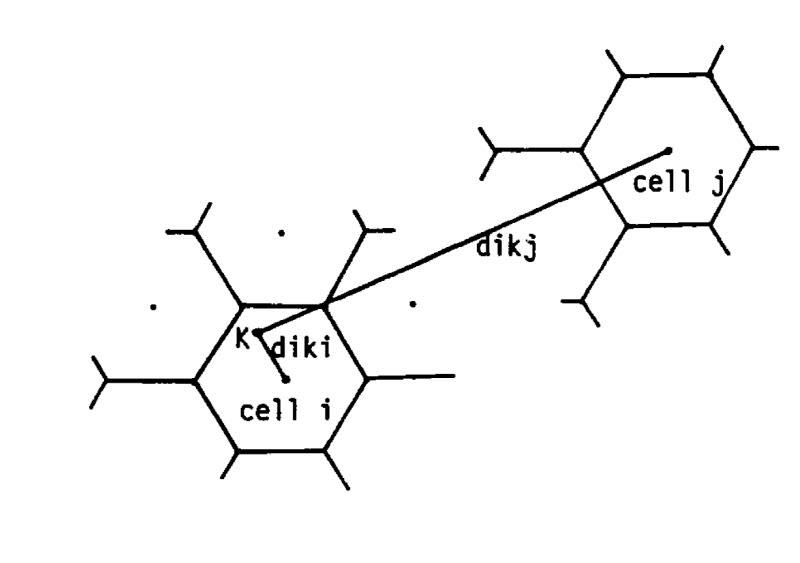
\includegraphics[scale=0.3]{t}
	\caption{Uplink and downlink interference geometry.}
	\label{fig:t}
\end{figure}

Abviously, it's easy to know that
\begin{equation}
P^{D}_{ik} = d^\alpha_{iki}P_i^D
\end{equation}
In an actual implementation, it would probably be more difficult to acquire the control information state for each user due to their motions. However, the model is convenient for the initial simulation.

We have neglected the effects of shadow fading in this work, which leads to an optimistic results. We will add the fading at next step.

6. \textit{Proposition:}There exists a unique maximum achievable SIR level:
\begin{equation*}
\qquad \gamma^{*} = \max\{\gamma | \exists P\geq 0 : \Gamma_i \geq \gamma, \forall i \}
\end{equation*}

%The maximum is given by  
%\begin{equation*}
%\gamma^{*} = \frac{1}{\lambda^{*}-1},
%\end{equation*}
%where $\lambda^*$ is the largest real eigenvalue of the matrix %max eigenvalue

For the uplink, the total power received by the base station express as:\begin{equation}
P_{sum} = \sum_{j=1}^N P_j^U \sum_{k=1}^{L_j} \left[ \frac{d_{jkj}}{d_{jki}}\right] ^{\alpha}
\end{equation}
The signal from the users thus suffer the signal-to-interference ration at the base station:
\begin{equation*}
\Gamma_i^U = \frac{P_i^U}{P_{sum}-P_i^U}
\end{equation*}.
Hence,
\begin{equation}
\frac{1+\gamma_i^U}{\gamma_i^U}P_i^U = \sum_{j=1}^N P_j^U \sum_{k=1}^{L_j} \left[\frac{d_jkj}{d_jki}\right] ^{\alpha}
\end{equation}
To balance the SIR for each user in cell i, and set all the SIR  in cell i to be equal, and solve the $P_i^U$for all i, then we can get the desired signal in the uplink by(4). This needs the solution of linear algebraic equation. We define this operation as in-cell balancing because different cells may have different $SIR^U$ values.

To get the $SIR^U$ for all cells, we should know that:
\begin{align}
P^U =& \left[ P^U_1, P^U_2,\dots,P^U_N \right]^T; \nonumber \\
G^U =& \left[ g^U_{ij}\times a_{ij}^U\right], where \ g^U_{ij} = \sum_{k=1}^{L_j} \left[ \frac{d_{jkj}}{d_{jki}}\right] ^{\alpha}
\end{align}
Since we neglected the shadow fading, the factor $a_{ij^U}$ can be set as 1. And now we have:
\begin{equation}
\ G^UP^U = \frac{1+\gamma^U}{\gamma^U}P^U
\end{equation}
as showed in (1).
Thus, we have the relationship between the SIR and the eigenvalue:
\begin{equation}
\lambda^U = \frac{1+\gamma^U}{\gamma^U}
\end{equation}
Then we convert the three-dimension control information to the two-dimension matrix problems, which is a classic eigenvalue problem with a eigenvector of $P^U$. 

The downlink's situation seems like it is in the uplink. We can talk about it later. The downlink's gain link matrix is a transpose of the uplink matrix, so that they have the same eigenvalue. 


\section{The Optimal Centralized Power Control Algorithm}
Let us consider a power control algorithm of the uplink, which has the uplinlk gain matrix G and may control the power vector P instantaneously. And assume that the transmission system requires a minimum (threshold) SIR $\gamma_0^U$. Jander assumed a method in order to minimizes the interference probability[2].


\vspace*{3mm}
Up to now, it caused a problem because of the matrix' composition. Each row or column consists of a whole cell's gain link information, while the removal of whole cell results in a worse case by the algorithm. We transform the link gain matrix from BS$\times $BS to user$\times$user. We set a CDMA system consisting of N cells with $L_k$ users in the k-th cell,and the total number is n. If the i-th user is m-th user in the k-th cell, we can get that:
\begin{equation}
i=\sum^k_{num=1}L_{num-1}+m \qquad 1\leq m\leq L_{num}
\end{equation}  

where $L_0$ = 0, $L_k$(n = 1,2,...,N) is the number of active users in cell K at one moment. By using the equations, we can derive the uplink SIR matrix for mobile i in cell k by (2)~(9):
\begin{equation}
\gamma_i^U = \frac{g_{ik}P_i}{ \sum_{j\neq i}g_{jk}P_j}
\end{equation}

We defind $G_{ij}$ = $\frac{g_{jk}}{g_{ik}}$, so that we can get the G matrix as:
\begin{equation}
\gamma_i^U = \frac{P_i}{ \sum_{j\neq i}G_{jk}P_j}
\end{equation}

Proof:There is at least one optimum power vector$ P^*$ satisfy the demend of the PCA, and then it has the form:
\begin{equation*}
P_i^{U} = P_i^{*U}, i \neq k; P_k^U=0.
\end{equation*}
We can obtain the SIR value by equation(12):

\begin{align*}
\gamma_i^U &= \frac{P_i^U}{\sum_{j=1}^{n}P_j^UG^U_{ij}-P^U_i} =\frac{P_I^{*U}}{\sum_{j=1}^{n}P_j^{*U}G^U_{ij}-P^{*U}_i-P^{*U}_kG^U_{ik}}	\\
&\geq \gamma_i^{*U}\geq \gamma_0, i \neq k.
\end{align*}	

P achieves a SIR that is not less than $\gamma_0$ while this is absolutely  achieved by $P^*$. Therefore, P is also an optimal vector. SO the removal will leads to a better SIR rather than make it decreased. 

Besides, there is a new algorithm, which is called SRA, will need n eigenvalue computations in the worst case, while it will cost $n^2$ times roughly by removing the user freely. This action means the BS cannot maintain the communication among the exist users, so we need to canceled the user or set up a new BS for the demands.

\vspace*{3mm}
\textbf{Stepwise Removal Algorithm$\left( \textbf{SRA} \right)$}              

(1)Step 1: Determine $\gamma^*$ corresponding to G. if $\gamma^*$ $\geq$ $\gamma^U_0$, then use the eigenvector $P^*$ and stop; else set N'=N and follow step 2.

(2)Step 2: Remove cell i for which the maximum of th row and colunm sums
\begin{align*}
r_k = \sum_{j=1}^{n} G^{U'}_{kj}\\
r_k^{T} = \sum_{j=1}^{n} G^{U'}_{jk}
\end{align*}
is maximized and form the (Q'-1) $\times$ (Q'-1) matrix G'. Determine the $\gamma^*$ correspoding to G' by(9) ,where $\gamma^*$ is the minimum of the SIR we can get, Furthermore, if the $\gamma^*$ is still bigger than the limitation, of which can maintain the communication, use the eigenvector $P^*$, else set Q' = Q'-1, and repeat step 2.

\textbf{Stepwise Maximum-Inteference Removal Algorithm $\left( \textbf{SMIRA} \right)$}              
The SMIRA is the same like SRA except the step 2, user k is removed if the maximum fo the sums 
\begin{equation}
r_k = \sum_{j=1}^{n}G^{U'}_{kj}P_j,\qquad r_k^{T} = \sum_{j=1}^{n}G^{U'}_{jk}P_k
\end{equation}
is maximized.

$r_k$ represents the total interference for user k in the uplink and $r_k^T$ of it represents the total interference to other users caused by user k[6], although they cannot represent these two concept exactly.  

\section{Numerical Result}

Tips:
1.we need the result of the simulation among the system without PCA, with in-cell PCA and with global PCA. Then we find that set all cell to be equal has the best performance, that can provide more users per cell.

2.Then we can compared the SRA with SMIRA, to find the probability of outage. And then use the better algorithm in step 1.

3.If there are n users without their state information, we choose the nearest BS for the user, and do the step 1. Then we change the user's BS if the $\gamma$ is lower than the limitation. 


\section{Conclusion}
The conclusion goes here.



% conference papers do not normally have an appendix


% use section* for acknowledgment
\section*{Acknowledgment}


The authors would like to thank...





% trigger a \newpage just before the given reference
% number - used to balance the columns on the last page
% adjust value as needed - may need to be readjusted if
% the document is modified later
%\IEEEtriggeratref{8}
% The "triggered" command can be changed if desired:
%\IEEEtriggercmd{\enlargethispage{-5in}}

% references section

% can use a bibliography generated by BibTeX as a .bbl file
% BibTeX documentation can be easily obtained at:
% http://mirror.ctan.org/biblio/bibtex/contrib/doc/
% The IEEEtran BibTeX style support page is at:
% http://www.michaelshell.org/tex/ieeetran/bibtex/
%\bibliographystyle{IEEEtran}
% argument is your BibTeX string definitions and bibliography database(s)
%\bibliography{IEEEabrv,../bib/paper}
%
% <OR> manually copy in the resultant .bbl file
% set second argument of \begin to the number of references
% (used to reserve space for the reference number labels box)
\begin{thebibliography}{1}

\bibitem{IEEEhowto:kopka}
R. W. Nettleton and H. Alavi, “Power control for a spread spectrum cellular mobile radio system,” in Proc., IEEE VTC., pp. 242–246, 1983. 
\bibitem{IEEEhowto:kopka}
J. Zander, “Performance of optimum transmitter power control in cellular radio systems,” IEEE Trans. Veh. Tech., vol. 41, no. 1, pp. 57–62, 1992.
\bibitem{IEEEhowto:kopka}
S. Grandhi, J. Zander, and R. D. Yates, “Constrained power control,” Int. J. of Wireless Pers. Comm., vol. 1, no. 4, 1995.
\bibitem{IEEEhowto:kopka}
Q. Wu, “Centralized power control in CDMA cellular mobile systems ,” IEEE 47th VTC., vol. 2, pp. 1268-1271, 1997.
\bibitem{IEEEhowto:kopka}
S. A. Grandhi and J. Zander, “Constrained power control in cellular radio systems,” in Proc., IEEE 44th VTC., vol. 2, pp. 824– 828, 1994. 
\bibitem{IEEEhowto:kopka}
S. A. Grandhi, R. Vijayan, D. J. Goodman, and J. Zander, “Centralized power control in cellular radio systems,” IEEE Trans. Veh. Tech., vol. 42, no. 4, pp. 466–468, 1993.
\bibitem{IEEEhowto:kopka}
Q. Wu, “Performance of optimum transmitter power control in CDMA cellular mobile systems,” IEEE Trans. Veh. Tech., vol. 48, no. 2, pp. 571–575, 1999.
\end{thebibliography}


% that's all folks
\end{document}
%\begin{abstract}
%BDMA can select the best beam for each user by analog beamforming. In this paper, we consider the digital precoding to improve the performance of hybrid beamforming MIMO system.
%\end{abstract}
%
%\section{Problem Formulation}
%Although BDMA has good performance on multi-path multi-user MIMO system, it supposes the infinite antennas of transmitter and only considers the analog beamforming. For hybrid beamforming system, we are enable to use digital precoding to eliminate the interference between users who are too close.
%
%For ULA transmitter, the channel model is expressed by
%\begin{equation}{\label{eq:Hu}}
%\bm{H}_u = \sqrt{\frac{N_{T}N_{R}}{L_{u}}}\sum_{l=1}^{L_u}\alpha_{u,l}\cdot \bm{a}_{R}(\phi^r_{u,l}) \cdot\bm{a}_{T}^{H}(\phi^t_{u,l}),
%\end{equation}
%
%The number of antennas is $N_T$ in transmitter. For infinite antennas of analog beamforming
%\begin{equation}
%\lim_{N_T\rightarrow \infty} \bm{a}_{T}^{*}(\alpha)\cdot \bm{a}_{T}(\beta) = 0 \quad \text{for} \quad \alpha\not= \beta
%\end{equation}
%
%
%
%The u-th received signal of UE is
%\begin{align}{\label{eq:hats}}
%\hat{s}_u & = \bm{w}_u^H \bm{H}_{u} \bm{V} \bm{f}_{u} \bm{s} + \bm{w}_u^H \bm{\tilde{n}}_u \\
%& = \gamma \bm{w}_u^H  \{\sum_{l=1}^{L_u} \bm{a}_{R}(\phi^r_{u,l}) \bm{a}_{T}^{H}(\phi^t_{u,l})\}\bm{V} \bm{f}_{u} \bm{s} + \bm{w}_u^H \bm{\tilde{n}}_u
%\end{align}
%
%The analog beamformer $\bm{V}$ can be selected to be orthogonal with others so that the SINR can be maximized. The digital precoding can be calculated by zero forcing. 
%
%In the simulation, I set the number of users is 20 and the number of antennas in transmitter is 128. The digital precoding matrix $F$ is designed as block matrix based on the users scheduling.
%\begin{figure}[ht]
%	\begin{center}
%		\includegraphics[width=3in,height=2.5in]{Figure/20usersGreedy.jpg}
%		\caption{Comparison of scheduling.}\label{fig:SpectralEffNoSelection}
%	\end{center}
%\end{figure}
%
%Although we assume the infinite antennas will result in the orthogonal steering vectors, the  $\bm{a}_{T}^{*}(\alpha)\cdot \bm{a}_{T}(\beta) \not= 0$ in practical, especially when the number of antennas is not large enough.
%
%
%\section{Clusters Perpendicular}
%
%\begin{figure}[h!]
%	\centering
%	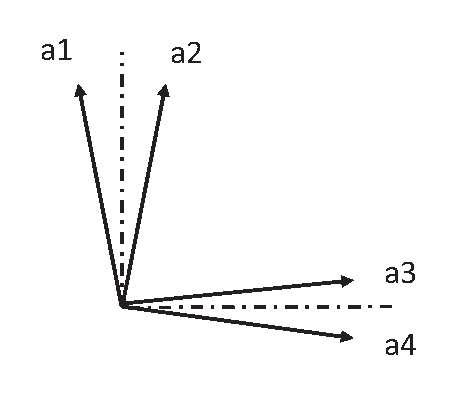
\includegraphics[width=2in]{Figure/Signal.eps}
%	\caption{Consider a case that there are two clusters which perpendicular to each other.}\label{fig:6}
%\end{figure}
%According the former discussion, we now design a perpendicular-cluster system to support more users by sharing same RF chain in one cluster.
%In this case, the number fo RF chains is 2, and the number of users is 4. Let's classify the 4 users to 2 cluster and $S_1,S_3$ is approximately orthogonal to $S_2,S4$ as shown in Fig.2. The arrows represent the AoDs of users. We use the analog precoding $F_{RF}$ to distinguish the clusters and use digital shared precoding $F_{BB}$ to separate the users in one cluster.
%
%Firstly, we design the baseband digital precoding matrix with $2N_{RF}\times N_s$, i.e. $4\times 4$ of $\mathbf{F_{BB}}$ as
%\begin{equation}
%\mathbf{F}=
%\begin{bmatrix}
%\bm{f_{1}} & \bm{f_{2}}&\mathbf{0}&\bm{0}\\
%\mathbf{0}&\mathbf{0}&\bm{f_{3}} & \bm{f_{4}}\\
%\end{bmatrix}
%=
%\begin{bmatrix}
%f_{1,1} & f_{1,2}&0&0\\
%f_{2,1} & f_{2,2}&0&0\\
%0&0&f_{3,3} & f_{3,4}\\
%0&0&f_{4,3} & f_{4,4}\\
%\end{bmatrix}
%\end{equation}
%
%And the analog precoding $\mathbf{V}$ is
%\begin{equation}
%\mathbf{V}=
%\begin{bmatrix}
%\bm{v_1} & \bm{v_2}&\bm{v_3}&\bm{v_4}\\
%\end{bmatrix}
%=
%\begin{bmatrix}
%\mathbf{V_{1,2}} & \mathbf{V_{3,4}}\\
%\end{bmatrix}
%\end{equation}
%
%Where $\bm{v_u}$ is a vector $N_T\times 1$, and $\mathbf{F_{1,2}}$ and $\mathbf{F_{3,4}}$ are a matrix with $N_T\times 2$.
%
%Now, let's write the digital precoding on $\mathbf{s}$
%\begin{equation}
%\mathbf{Fs}=
%\begin{bmatrix}
%\bm{f_{1}} & \bm{f_{2}}&\bm{0}&\bm{0}\\
%\bm{0}&\bm{0}&\bm{f_{3}} & \bm{f_{4}}\\
%\end{bmatrix}
%\begin{bmatrix}
%s_1\\s_2\\s_3\\s_4
%\end{bmatrix}
%=
%\begin{bmatrix}
%\mathbf{f_{1}}s_1 + \mathbf{f_{2}}s_2\\
%\mathbf{f_{3}}s_3 + \mathbf{f_{4}}s_4\\
%\end{bmatrix}
%\end{equation}
%
%Then we implement the analog precoding on $\mathbf{F_{BB}s}$
%\begin{equation}
%\mathbf{VFs}= \mathbf{V_{1,2}}\bm{f_1}s_1+\mathbf{V_{1,2}}\bm{f_2}s_2 + \mathbf{V_{3,4}}\bm{f_3}s_3+\mathbf{V_{3,4}}\bm{f_4}s_4
%\end{equation}
%And the received processed signal is
%
%\begin{equation}
%\hat{s}_u = \mathbf{w_u^H H_u}[\mathbf{V_{1,2}}(\bm{f_1}s_1+\bm{f_2}s_2) +\mathbf{V_{3,4}}(\bm{f_3}s_3+\bm{f_4}s_4)]+ \mathbf{w_u^H n_u}
%\end{equation}
%
%Thus, we need to design $\mathbf{F}$ to minimize the interference.
%
% we want $\mathbf{w_u H_u V F}$  to be diagonal matrix.
%$$
%%\begin{equation}
%\begin{bmatrix}
%\mathbf{w_1^H H_1 V}\\\mathbf{w_2^H H_2 V}\\\mathbf{w_3^H H_3 V}\\\mathbf{w_4^H H_4 V}\\
%\end{bmatrix}
%\begin{bmatrix}
%\mathbf{F}\\
%\end{bmatrix}
%=\\
%\begin{bmatrix}
%\mathbf{w_1^H H_1 [V_{1,2}\quad V_{3,4}]}\\\mathbf{w_2^H H_2 [V_{1,2}\quad V_{3,4}]}\\\mathbf{w_3^H H_3 [V_{1,2}\quad V_{3,4}]}\\\mathbf{w_4^H H_4 [V_{1,2}\quad V_{3,4}]}\\
%\end{bmatrix}
%\begin{bmatrix}
%\bm{f_{1}} & \bm{f_{2}}&\mathbf{0}&\mathbf{0}\\
%\bm{0}&\bm{0}&\bm{f_{3}} & \bm{f_{4}}\\
%\end{bmatrix}
%$$
%%\begin{bmatrix}
%%\mathbf{\mathbf{he_1}}\\\mathbf{he_2}\\\mathbf{he_3}\\\mathbf{he_4}\\
%%\end{bmatrix}
%%\begin{bmatrix}
%%\mathbf{f_{1}^{BB}} & \mathbf{f_{2}^{BB}}&\mathbf{f_{3}^{BB}} & \mathbf{f_{4}^{BB}}\\
%%\end{bmatrix}
%%\end{equation}
%
%
%\begin{equation}
%=
%\begin{bmatrix}
%\mathbf{w_1^H H_1 V_{1,2} f_1}&\mathbf{w_1^H H_1 V_{1,2} f_2}&\mathbf{w_1^H H_1 V_{3,4} f_3}&\mathbf{w_1^H H_1 V_{3,4} f_4}\\
%\mathbf{w_2^H H_2 V_{1,2} f_1}&\mathbf{w_2^H H_2 V_{1,2} f_2}&\mathbf{w_2^H H_2 V_{3,4} f_3}&\mathbf{w_2^H H_2 V_{3,4} f_4}\\
%\mathbf{w_3^H H_3 V_{1,2} f_1}&\mathbf{w_3^H H_3 V_{1,2} f_2}&\mathbf{w_3^H H_3 V_{3,4} f_3}&\mathbf{w_3^H H_3 V_{3,4} f_4}\\
%\mathbf{w_4^H H_4 V_{1,2} f_1}&\mathbf{w_4^H H_4 V_{1,2} f_2}&\mathbf{w_4^H H_4 V_{3,4} f_3}&\mathbf{w_4^H H_4 V_{3,4} f_4}\\
%\end{bmatrix}
%%\begin{bmatrix}
%%\mathbf{he_1 f_{1,1}^{BB}}&0&\mathbf{he_1f_{3}^{BB}}&0\\
%%0&\mathbf{he_2 f_{2}^{BB}}&0&\mathbf{he_2 f_{4}^{BB}}\\
%%\mathbf{he_3 f_{1}^{BB}}&0&\mathbf{he_3 f_{3}^{BB}}&0\\
%%0&\mathbf{he_4 f_{2}^{BB}}&0&\mathbf{he_4 f_{4}^{BB}}\\
%%\end{bmatrix}
%\end{equation}
%
%
%From the channel model, we have $\mathbf{H_u = a_R(u)D(u)a_T^H(u)}$ for LOS channel. As shown in \figurename{6}, we know that $$AoD_{a1}\approx AoD_{a_2} \perp AoD_{a3}\approx AoD_{a4}$$
%
%Therefore,
%$$
%\mathbf{H_1 V_{3,4}=H_2 V_{3,4}=0} ,\quad \mathbf{H_3 V_{1,2}=H_4 V_{1,2}=0}
%$$
%And we can rewrite the expression of transeiver system
%\begin{equation}
%\mathbf{w_u H_u V F}=
%\begin{bmatrix}
%\mathbf{w_1^H H_1 V_{1,2} f_1}&\mathbf{w_1^H H_1 V_{1,2} f_2}&0&0\\
%\mathbf{w_2^H H_2 V_{1,2} f_1}&\mathbf{w_2^H H_2 V_{1,2} f_2}&0&0\\
%0&0&\mathbf{w_3^H H_3 V_{3,4} f_3}&\mathbf{w_3^H H_3 V_{3,4} f_4}\\
%0&0&\mathbf{w_4^H H_4 V_{3,4} f_3}&\mathbf{w_4^H H_4 V_{3,4} f_4}\\
%\end{bmatrix}
%\end{equation}
%%\begin{equation}
%%\mathbf{w_u H_u F_{RF} F_{BB}}=
%%\begin{bmatrix}
%%\mathbf{w_1^H H_1 a_1}f_{1,1}^{BB}&\mathbf{w_1^H H_1 a_1} f_{2,1}^{BB}&\mathbf{w_1^H H_1 a_1}f_{3,1}^{BB}&\mathbf{w_1^H H_1 a_1} f_{4,1}^{BB}\\
%%\mathbf{w_2^H H_2 a_2}f_{1,2}^{BB}&\mathbf{w_2^H H_2 a_2} f_{2,2}^{BB}&\mathbf{w_2^H H_2 a_2}f_{3,1}^{BB}&\mathbf{w_2^H H_2 a_2} f_{4,2}^{BB}\\
%%\mathbf{w_1^H H_1 a_1}f_{1,1}^{BB}&\mathbf{w_1^H H_1 a_1} f_{2,1}^{BB}&\mathbf{w_1^H H_1 a_3}f_{3,1}^{BB}&\mathbf{w_1^H H_1 a_1} f_{4,1}^{BB}\\
%%\mathbf{w_1^H H_1 a_1}f_{1,1}^{BB}&\mathbf{w_1^H H_1 a_1} f_{2,1}^{BB}&\mathbf{w_1^H H_1 a_3}f_{3,1}^{BB}&\mathbf{w_1^H H_1 a_1} f_{4,1}^{BB}\\
%%\end{bmatrix}
%%\end{equation}
%%The processed signal is
%%\begin{equation}
%%\mathbf{\hat{S}}=
%%\begin{bmatrix}
%%\mathbf{w_1^H H_1 F_{1,2}^{RF} f_1^{BB}}s_1+\mathbf{w_1^H H_1 F_{3,4}^{RF} f_3^{BB}}s_3\\
%%\mathbf{w_2^H H_2 F_{1,2}^{RF} f_2^{BB}}s_2+\mathbf{w_2^H H_2 F_{3,4}^{RF} f_4^{BB}}s_4\\
%%\mathbf{w_3^H H_3 F_{1,2}^{RF} f_1^{BB}}s_1+\mathbf{w_3^H H_3 F_{3,4}^{RF} f_3^{BB}}s_3\\
%%\mathbf{w_4^H H_4 F_{1,2}^{RF} f_2^{BB}}s_2+\mathbf{w_4^H H_4 F_{3,4}^{RF} f_4^{BB}}s_4\\
%%\end{bmatrix}
%%\end{equation}
%
%
%Let's focus on $\mathbf{f_1}$ and $\mathbf{f_2}$ to eliminate the interference.
%\begin{equation}
%\begin{bmatrix}
%\mathbf{w_1^H H_1 V_{1,2} f_1}&\mathbf{w_1^H H_1 V_{1,2} f_2}\\
%\mathbf{w_2^H H_2 V_{1,2} f_1}&\mathbf{w_2^H H_2 V_{1,2} f_2}\\
%\end{bmatrix}
%=
%\begin{bmatrix}
%\mathbf{w_1^H H_1 V_{1,2}}\\\mathbf{w_2^H H_2 V_{1,2}}\\
%\end{bmatrix}
%\begin{bmatrix}
%\mathbf{f_1}  &  \mathbf{f_2}
%\end{bmatrix}
%=
%\mathbf{H^{eq}_{1,2} F_{1,2}}=\mathbf{I}
%\end{equation}
%
%Similarly, $\mathbf{H^{eq}_{3,4} F_{3,4}}=\mathbf{I}$

%\section{Single Path}
%In our previous work, we use channel model with single path for simplicity. The channel model is given by
%
%\begin{equation}{\label{eq:HuLu1}}
%\bm{H}_u = \sqrt{N_{T}N_{R}}\cdot\alpha_u \cdot\bm{a}_{R}(\phi^r_{u},\theta^r_{u})\cdot\bm{a}^{H}_{T}(\phi^t_{u},\theta^t_{u}).
%\end{equation}
%
%In each simulation iteration, several users (\textit{i.e.} 4 users) will be selected to serve and the others will be ignored. However, it's unrealistic for any environment and unreasonable to ignore some users under base station.
%
%\section{Multi-path Channel Model}
%By considering the assumption of BDMA, the channel model is represented as 
%
%\begin{equation}{\label{eq:Hu}}
%\bm{H}_u = \sqrt{\frac{N_{T}N_{R}}{L_{u}}}\sum_{l=1}^{L_u}\alpha_{u,l}\cdot \bm{a}_{R}(\phi^r_{u,l},\theta^r_{u,l}) \cdot\bm{a}_{T}^{H}(\phi^t_{u,l},\theta^t_{u,l}),
%\end{equation}
%and
%\begin{equation}
%	\lim_{N\rightarrow \infty} \bm{e}_t^H(\phi) \bm{e}_t(\eta) = \delta(\phi-\eta)
%\end{equation}
%where $N$ is the number of transmitter antennas.
%
%\subsection{Analog-only BDMA beamforming}
%For the analog-only problem, the opportunity will increase with increased paths. However, the interference will also increase since the several paths of channel model as shown in the following equation
%\begin{align}
%\text{single path:} I_u &= \sum_{i\not=u}^{N_U} ||w_u H_u v_i||^2_F =\sum_{i\not=u}^{N_U} ||w_u a_R a^H_T v_i||^2_F \nonumber\\
%\text{$L_u$ paths:} I_u &= \sum_{i\not=u}^{N_U} ||w_u H_u v_i||^2_F =\sum_{i\not=u}^{N_U} ||w_u \sum_{l}^{L_u}a_R^l (a^l_T)^H v_i||^2_F
%\end{align}
%Where $v_i$ is the analog beamforming vector of $i$th user.
%
%
%\subsection{Zero-forcing still works in multipath channel model}
%
%Although analog-only BDMA can significantly improve the capacity, the interference of different users can be totally eliminated, which means
%\begin{align}
%   S_u &= ||w_u H_u V f_u||^2_F \not= 0 \\\label{zeroforcing}
%   I_u &= \sum_{i\not=u}^{N_u}||w_u H_u V f_i||=0 
%\end{align}
%
%\section{The user scheduling for block diagonal matrix optimization }
%Our objective is to transform the digital precoding matrix $F\in \mathcal{C}^{N_U\times N_U}$ to a block diagonal matrix $F = diag(F_1,F_2,\cdots,F_K)$. Then, the number of RF chains can be reduced to $N_u/K$ by applying TDD.
%
%In the basic idea, we use analog beamforming to eliminate the interference between different cluster and digital precoding to eliminate the interference in same cluster.
%
%The greedy algorithm can be written as follows:\\
%1. Choose 1st user randomly. Group1 contains \{user1\}.\\
%2. Calculate for all users and choose 2nd user that has \textbf{maximal} interference on Group1. Group1 contains \{user1, user2\}.\\
%3. Repeat step 2 and stop assigning for group1 until the number of members in group1 is equal to $N_u/K$. \\
%4. Calculate for the left users and choose the user1 for group2 with \textbf{minimal} interference on Group1. Group2 contains \{user1\}\\
%5. Repeat the steps above, all the users can be scheduled.
%
%\subsection{Clipping on the off-block-diagonal elements}
%The simplest way to implement block diagonal digital precoding is manually setting all the off-block-diagonal elements to be zero. However, the interference will increase since $I_u\not=0$ in eq.\ref{zeroforcing} .
%
%\subsection{User scheduling and clipping on off-block-diagonal elements}
%If the block matrix is transformed by user scheduling, the off-block-diagonal elements has least interference on others.
%
%\subsection{User scheduling and convex optimization algorithm}
%After user scheduling, We set the constraints on digital precoding and then solve the optimal $F$ by minimizing the difference with zero-forcing upper bound $F_{ZF}$.
%\begin{flalign}\label{eq:optdigPreMatPAPR}
%F &= \argmin ||He*F - He*F_{ZF}||_F^2\\
%s.t. \quad &\text{the off-block-diagonal-matrix elements of $F$ are 0}
%\end{flalign}
%
%
%\section{Simulation for single path}
%
%\subsection{signle-path channel model}
%\begin{figure}[H]
%	\begin{center}
%		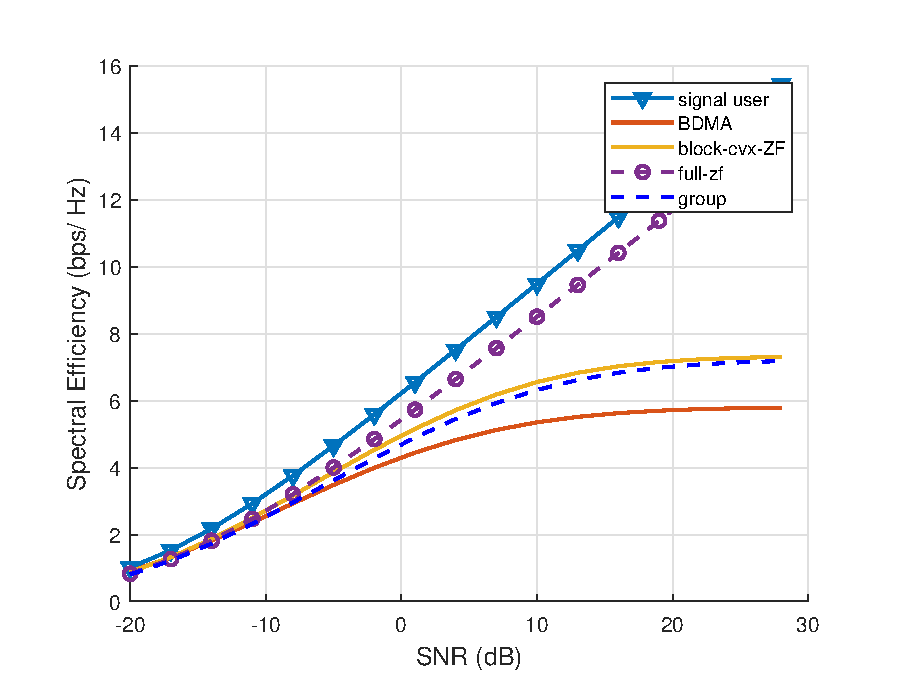
\includegraphics[scale=0.7]{Figure/16singlepath}
%		\caption{16 users with 1 path for each user. The digital precoding matrix is divided into 4$\times$4} block-diagonal matrix\label{single}
%	\end{center}
%\end{figure}
%
%\subsection{Multi-path channel model }
%\begin{figure}[H]
%	\begin{center}
%		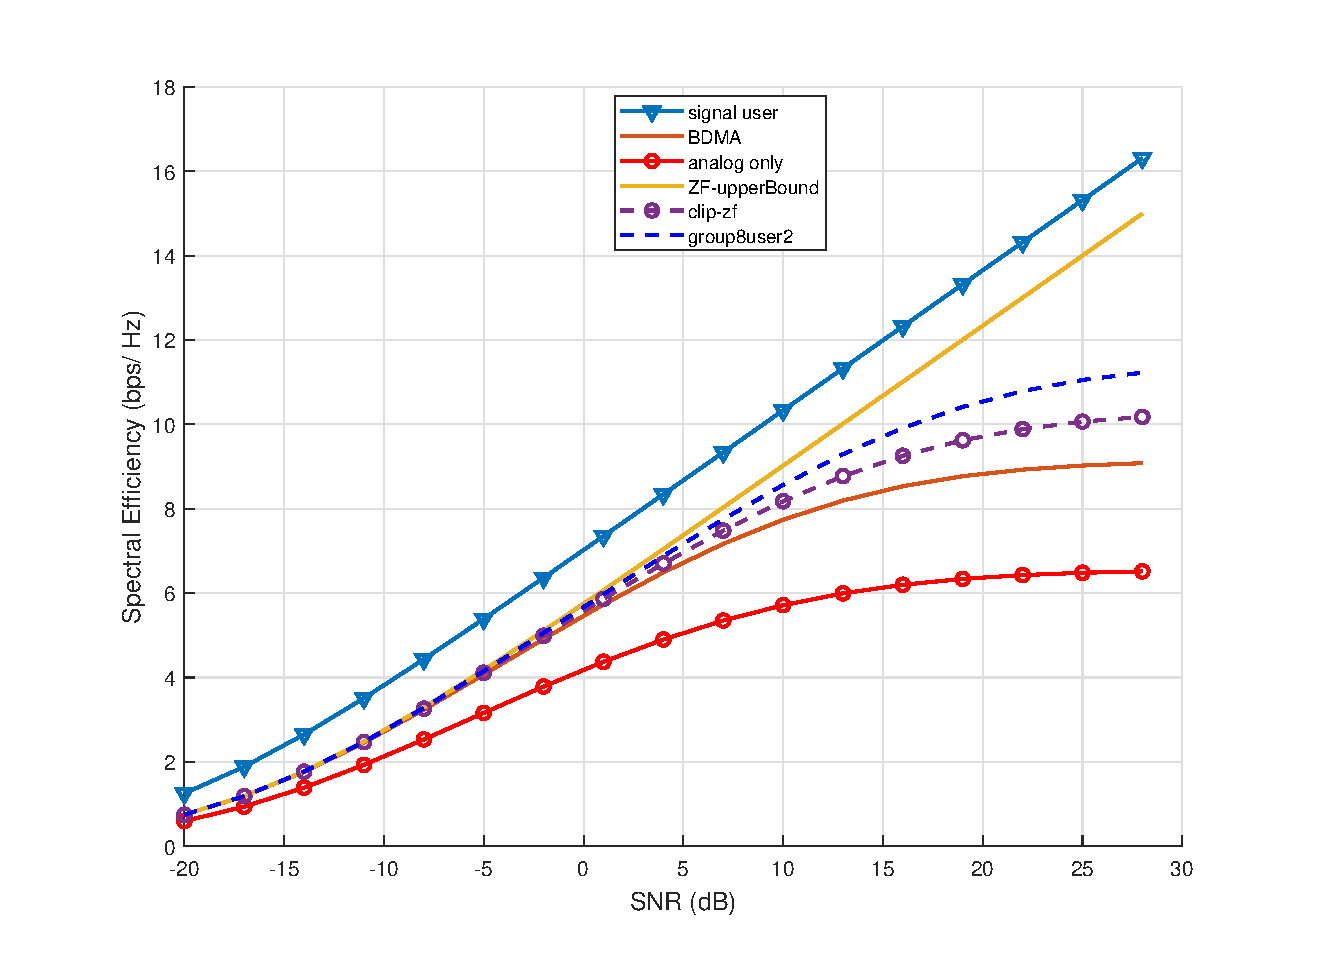
\includegraphics[scale=0.5]{Figure/8usercomparisonWithGroup}
%		\caption{8 users with 4 paths for each user. The digital precoding matrix is divided into 4$\times$2.} \label{multiusers}
%	\end{center}
%\end{figure}
%
%\begin{figure}[H]
%	\begin{center}
%		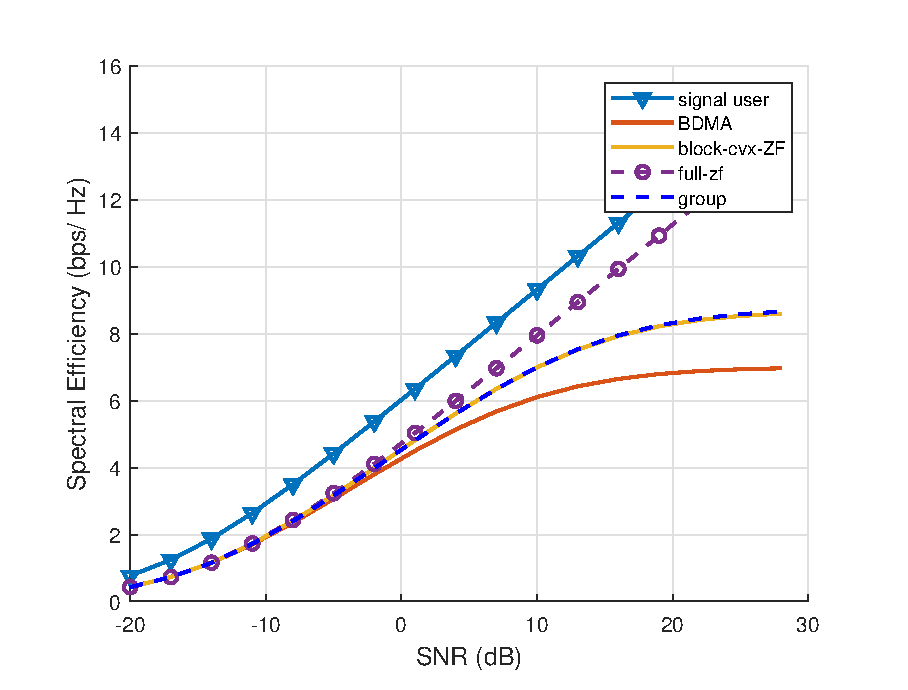
\includegraphics[scale=0.7]{Figure/16users4pathBlock}
%		\caption{16 users with 4 paths for each user. The digital precoding matrix is divided into 4$\times$2.} 
%	\end{center}
%\end{figure}
%
%\subsection{Comparison of different number of paths for each user}
%\begin{figure}[H]
%	\begin{center}
%		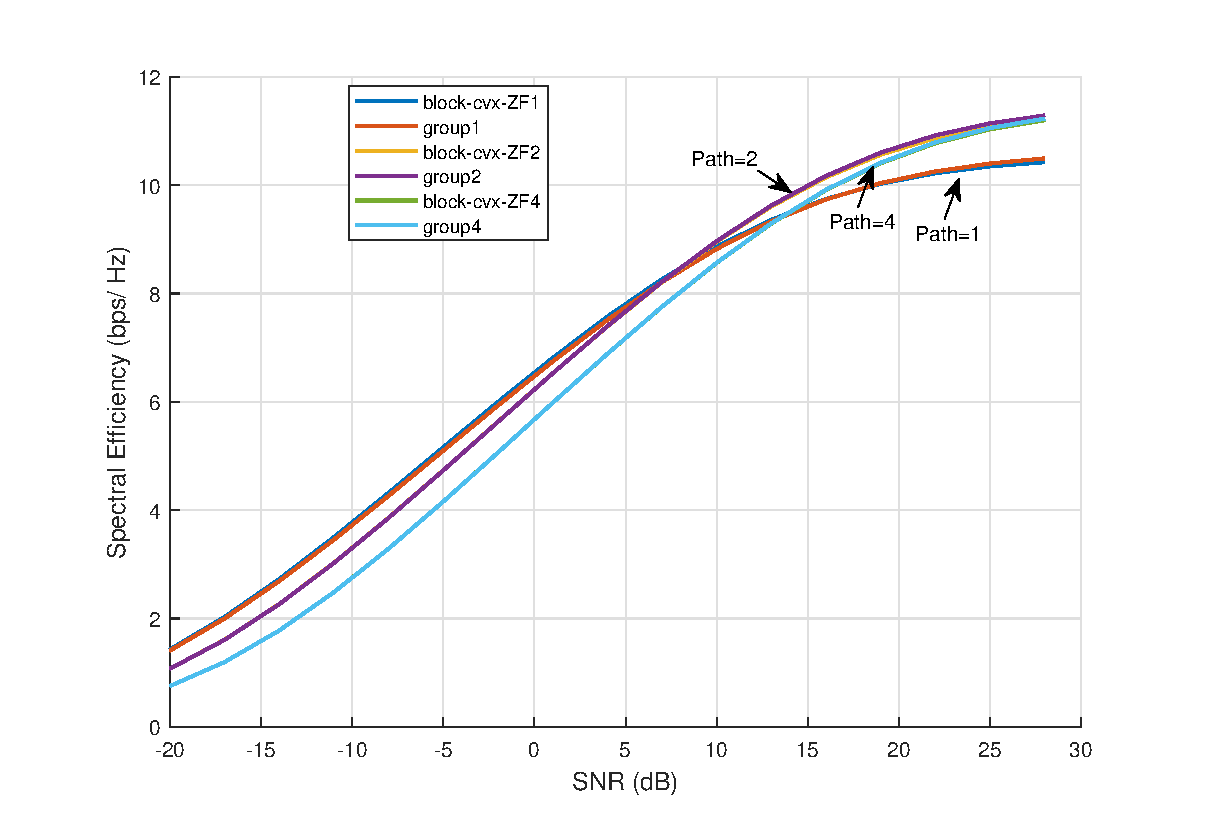
\includegraphics[scale=0.6]{Figure/1-2-4path}
%		\caption{comparison of 8 users with different paths.} 
%	\end{center}
%\end{figure}
%
%% references section
%%\bibliography{BDMAref}
%\bibliographystyle{IEEEtran}
%\end{document}


